\documentclass[hidelinks]{article}

\usepackage[sensei=Nakahara,gakka=Geometry\ in\ Physics,section=Quantum,gakkabbr=QM]{styles/kurisuen}
\usepackage{sidenotes}
\usepackage{van-de-la-sehen-en}
\usepackage{van-de-environnement-en}
\usepackage{boite/van-de-boite-en}
\usepackage{van-de-abbreviation}
\usepackage{van-de-neko}
\usepackage{van-le-trompe-loeil}
\usepackage{cyanide/van-de-cyanide}
\setlength{\parindent}{0pt}
\usepackage{enumitem}
\newlist{citemize}{itemize}{3}
\setlist[citemize,1]{noitemsep,topsep=0pt,label={-},leftmargin=1em}

\usepackage{mathtools}
\usepackage{ragged2e}

\DeclarePairedDelimiter\abs{\lvert}{\rvert}%
\DeclarePairedDelimiter\norm{\lVert}{\rVert}%

% Swap the definition of \abs* and \norm*, so that \abs
% and \norm resizes the size of the brackets, and the 
% starred version does not.
\makeatletter
\let\oldabs\abs
\def\abs{\@ifstar{\oldabs}{\oldabs*}}
%
\let\oldnorm\norm
\def\norm{\@ifstar{\oldnorm}{\oldnorm*}}
\makeatother

\newcommand*{\Value}{\frac{1}{2}x^2}%

\usepackage{fancyhdr}
\usepackage{lastpage}

\fancypagestyle{plain}{%
\fancyhf{} % clear all header and footer fields
\fancyhead[R]{\smash{\raisebox{2.75em}{{\hspace{1cm}\color{lightgray}\textsf{\rightmark\quad Page \thepage/\pageref{LastPage}}}}}} %RO=right odd, RE=right even
\renewcommand{\headrulewidth}{0pt}
\renewcommand{\footrulewidth}{0pt}}
\pagestyle{plain}

\newtheorem*{experiment*}{Measurement}
\newtheorem{example}{Example}
\newtheorem{remark}{Remark}

\def\elementcell#1#2#3#4#5#6#7{%
    \draw node[draw, regular polygon, regular polygon sides=4, minimum height=2cm, draw=cyan, line width=0.4mm, fill=cyan!15!white, #1, inner sep=-2mm](#3) {\Large\textbf{\textsf{\color{cyan!50!black}#4}}};
    \draw (#3.corner 1) node[below left] {\footnotesize{\phantom{Hj}#5}};
    \draw (#3.corner 2) node[below right] {\small{\textsf{#6}}};
    \draw (#3.side 3) node[above] {\footnotesize #7};
    \draw (#3.corner 2) ++ (0,-0.4mm) node(nw#3) {};
    \tcbsetmacrotowidthofnode{\elementcellwidth}{#3}
    \node [fill=cyan, line width=0mm, rectangle, rounded corners=1.8mm, rectangle round south east=false, rectangle round south west=false, anchor=south west, minimum width=\elementcellwidth] at (nw#3) {\small\textsf{\color{white}#2}};
}

\DeclareSIUnit\Dq{Dq}
\usepackage{physics}
\usepackage{bbm}
\newtheorem{lemma}{Lemma}
\newtheorem{proposition}{Proposition}

\DeclareMathOperator{\Pfaffian}{Pf}
\DeclareMathOperator{\sign}{sign}

\usepackage[super]{nth}

\usetikzlibrary{decorations.pathmorphing}

\tikzset{snake it/.style={decorate, decoration=snake}}

\usepackage{stackengine}
\stackMath
\usepackage{scalerel}
\usepackage[outline]{contour}

\newlength\thisletterwidth
\newlength\gletterwidth
\newcommand{\leftrightharpoonup}[1]{%
{\ooalign{$\scriptstyle\leftharpoonup$\cr%\kern\dimexpr\thisletterwidth-\gletterwidth\relax
$\scriptstyle\rightharpoonup$\cr}}\relax%
}
\def\tensorb#1{\settowidth\thisletterwidth{$\mathbf{#1}$}\settowidth\gletterwidth{$\mathbf{g}$}\stackon[-0.1ex]{\mathbf{#1}}{\boldsymbol{\leftrightharpoonup{#1}}}  }
\def\onedot{$\mathsurround0pt\ldotp$}
\def\cddot{% two dots stacked vertically
  \mathbin{\vcenter{\baselineskip.67ex
    \hbox{\onedot}\hbox{\onedot}}%
  }}%

\begin{document}

\section{Semiconductors} % (fold)
\label{sec:semiconductors}

\subsection{Band Structure} % (fold)
\label{sub:band_structure}

\subsubsection{Band Gap} % (fold)
\label{ssub:band_gap}

A band gap is called a \gloss{direct band gap} if the crystal momentum of electrons and holes is the same in both the conduction band and the valence band. Otherwise it is called an \gloss{indirect band gap}.
\par
In an excitation through a direct band gap, the conservation of momentum is written as $\hbar \+vk' - \hbar \+vk = \+vp_\gamma$, where $\+vp_\gamma$ is generally neglectable and therefore $\+vk' = \+vk$. In an excitation through a indirect band gap, a phonon must be emitted or absorbed, hence
\[ \hbar \+vh' - \hbar \+vk = \pm\hbar \+vq. \]

% subsubsection band_gap (end)

\subsubsection{Effect Mass at Band Edges} % (fold)
\label{ssub:effect_mass_at_band_edges}

The equation describing the Block wave $\psi_{n\+vk} = e^{i\+vk\cdot \+vr}u_{n\+vk}\pare{\+vr}$ is written
\[ \brac{\frac{\+vp^2}{2m} + V\pare{\+vr} + \frac{\hbar}{m}\+vk\cdot \+vp}u_{n\+vk}\pare{\+vr} = \pare{E_n\pare{\+vk} - \frac{\hbar^2 k^2}{2m}}u_{n\+vk}\pare{\+vr}, \]
whence, with the solution at the $\Gamma$ point, i.e. $\+vk = 0$ given as $u_{n0}\pare{\+vr}$ and via the second order perturbation theory, we find
\[ E_n\pare{\+vk} = E_n\pare{0} + \frac{\hbar^2 k^2}{2m} + \frac{\hbar^2}{m^2}\sum_i \sum_{n'} \frac{\bra{n0}p_j\ket{n'0}\bra{n'0}p_i\ket{n0}}{E_n\pare{0} - E'_n\pare{0}} k_i^2, \]
where the pricipal axes are chosen and terms linear in $k$ from the first-order perturbation are discarded since we are only concerned about the behaviour near the extrema.
\par
If the extremum lies at some $\+vk_0 \neq 0$, the above approximation still applies.
\begin{finaleq}{Effective Mass at Band Edges}
    \[ \rec{m^*} = \rec{m} + \frac{2}{m}\sum_{n'}\frac{\bra{n\+vk_0}p_i\ket{n'\+vk_0}\bra{n'\+vk_0}p_i\ket{n\+vk_0}}{E_n\pare{\+vk_0} - E'_n\pare{\+vk_0}}. \]
\end{finaleq}
The effective mass is generally anisotropic. The effective mass along the symmetry axis is the \gloss[-\baselineskip]{longitudinal effective mass} $m_l$, while the one perpendicular to the symmetry axis is the \gloss{transversal effective mass} $m_t$.
\par
In some cases there may be degeneracy near the extrema, and the effective mass model breaks down.

% subsubsection effect_mass_at_band_edges (end)

% subsection band_structure (end)

\subsection{Doping} % (fold)
\label{sub:doping}

\subsubsection{Donor and Acceptor} % (fold)
\label{ssub:donor_and_acceptor}

A dopant that holds bound electrons in the band gap is called a \gloss[-2\baselineskip]{donor}, while that offers empty level is called a \gloss[-2\baselineskip]{acceptor}. Those whose conductivity relies on the donors are \gloss[-2\baselineskip]{n-type semiconductor}, whole those that relies on the acceptors are \gloss{p-type semiconductor}.

% subsubsection donor_and_acceptor (end)

\subsubsection{Shallow Level Doping} % (fold)
\label{ssub:shallow_level_doping}

\paragraph{N-Type Doping} % (fold)
\label{par:n_type_doping}

The dopant is hydrogen-like, the wavefunction of the donor electron is given by
\[ \psi_d\pare{\+vr} = F\pare{\+vr}u_0\pare{\+vr} \]
where
\[ \brac{-\frac{\hbar^2}{2m^*}\grad^2 - \frac{q^2}{4\pi\epsilon r}}F\pare{\+vr} = E_d F\pare{\+vr}. \]
The groud state energy is given by
\[ \inlinefinaleq{E\+_i_ = \frac{m^*}{m}\pare{\rec{\epsilon_r}}^2E\+_H_,} \]
and the Bohr radius by
\[ \inlinefinaleq{a = \frac{m\epsilon_r}{m^*}a_0.} \]
The energy level is shallow and the wavefunction is extended.

% paragraph n_type_doping (end)

\paragraph{P-Type Doping} % (fold)
\label{par:p_type_doping}

There is one atom less, i.e. one hole more, in the valence band and one more negative charge at the site of doping.

% paragraph p_type_doping (end)

% subsubsection shallow_level_doping (end)

\subsubsection{Deep Level Doping} % (fold)
\label{ssub:deep_level_doping}

If the dopant creates a deep trap in the band gap, the doping is then a deep level one.

% subsubsection deep_level_doping (end)

% subsection doping (end)

\subsection{The Fermi-Dirac Distribution of Electrons} % (fold)
\label{sub:the_fermi_dirac_distribution_of_electrons}

\subsubsection{The Boltzmann Distribution Approximation} % (fold)
\label{ssub:the_boltzmann_distribution_approximation}

In a semiconductor, the band gap $E_- - E_+ \gg k\+_B_T$. Hence the occupancy of the electrons in the conduction band and the holes in the valence band is given by
\[ f\pare{E} \approx e^{-\pare{E-E\+_F_}/k\+_B_T}, \quad \text{and}\quad 1-f\pare{E} \approx e^{-\pare{E\+_F_ - E}/k\+_B_T}, \]
respectively.

% subsubsection the_boltzmann_distribution_approximation (end)

\subsubsection{Chaerge Carrier Density} % (fold)
\label{ssub:chaerge_carrier_density}

The densities of states at the band edges are given by
\[ N_-\pare{E} = \frac{4\pi\pare{2m^*_-}^{3/2}}{h^3}\sqrt{E-E_-},\quad \text{and}\quad N_+\pare{E} = \frac{4\pi\pare{2m^*_+}^{3/2}}{h^3}\sqrt{E_+ - E}. \]
The density of conduction electrons is therefore
\begin{equation}
    \label{eq:density_of_conduction_electrons}
    n = \int_{E_-}^\infty f\pare{E}N_-\pare{E}\,\rd{E} = N_- e^{-\pare{E_- - E\+_F_}/\pare{k\+_B_T}},
\end{equation}
where
\[ N_- = \frac{2\pare{2\pi m^*_- k\+_B_T}^{3/2}}{h^3} \]
is the effective density of level. The density of holes is similarly given by
\[ p = N_+ e^{-\pare{E\+_F_ - E_+}/\pare{k\+_B_T}}, \]
where
\[ N_+ = \frac{2\pare{2\pi m^*_+ k\+_B_T}^{3/2}}{h^3}. \]
\vspace{-\baselineskip}
\begin{finaleq}{Product of Densities}
    \begin{equation}
        \label{eq:product_of_densities}
        np = N_- N_+ e^{-\pare{E_- - E_+}/\pare{k\+_B_T}}.
    \end{equation}
\end{finaleq}

% subsubsection chaerge_carrier_density (end)

\subsubsection{Impurity Excitation} % (fold)
\label{ssub:impurity_excitation}

If the semiconductor is doped with donor of energy level $E_D$ and density $N_D$, the density of electrons is given by
\[ n = N_D \cdot \rec{1+e^{\pare{E\+_F_ - E\+_D_}/\pare{k\+_B_T}}} \xlongequal{\eqref{eq:density_of_conduction_electrons}} \frac{N_D}{\displaystyle 1+\frac{n}{N_-}e^{{E\+_i_}/\pare{k\+_B_T}}}. \]
If $E\+_i_ \gg k\+_B_T$, we have
\[ \inlinefinaleq{n \approx \sqrt{N_- N_D}e^{-E\+_i_/\pare{2k\+_B_T}},\quad \text{and}\quad p \approx \sqrt{N_A N_+} e^{-E\+_i_/\pare{2k\+_B_T}}.} \]
When $k\+_B_T \gg E\+_i_$ however, we have
\[ n \approx N_D,\quad \text{and}\quad p \approx N_A. \]

% subsubsection impurity_excitation (end)

\subsubsection{Intrinsic Excitation} % (fold)
\label{ssub:intrinsic_excitation}

For intrinsic excitation, $n \approx p$, from \eqref{eq:product_of_densities} we find
\begin{finaleq}{Intrinsic Excitation}
    \[ n\approx p = \sqrt{N_- N_+}e^{-E\+_g_/\pare{2k\+_B_T}},\quad \text{where}\quad E\+_g_ = E_- - E_+. \]
\end{finaleq}

% subsubsection intrinsic_excitation (end)

% subsection the_fermi_dirac_distribution_of_electrons (end)

\subsection{Transport Properties} % (fold)
\label{sub:transport_properties}

\subsubsection{Electrical Conductivity} % (fold)
\label{ssub:electrical_conductivity}

The electrical conductivity is given by
\[ \inlinefinaleq{\sigma = \begin{cases}
    nq\mu_-, & \text{n-type}, \\
    nq\mu_+, & \text{p-type}.
\end{cases}} \]
Plotting $\sigma$ against $1/T$ yields a U-shaped curve.
\par
For the \gloss{Hall effect} we have
\[ \inlinefinaleq{\frac{E_y}{B_z} = \begin{cases}
    \displaystyle -\rec{nq}j_x, & \text{n-type}, \\
    \displaystyle \rec{pq}j_x, & \text{p-type}.
\end{cases}} \]
The \gloss{Hall coefficient} is defined by
\[ \inlinefinaleq{R\+_H_ = \frac{E_y}{j_x B_z}.} \]

% subsubsection electrical_conductivity (end)

\subsubsection{Nonequilibrium Charge Carriers} % (fold)
\label{ssub:nonequilibrium_charge_carriers}

\paragraph{Nonequilibrium Carriers} % (fold)
\label{par:nonequilibrium_carriers}

Nonequilibrium charge carriers may be created, breaking the equilibrium condition \eqref{eq:product_of_densities}. $\Delta n = n-n_0$ and $\Delta p = p-p_0$ cancels each other to maintain the electrical neutrality.
\par
Recombination may occur between nonequilibrium charge carriers, with the rate
\[ \Delta n = \pare{\Delta n}_0 e^{-t/\tau}, \]
where $\tau$ is the life of the nonequilibrium carriers. During the recombination, electrons generally fall first into a empty impurity level, and then fall into the valence band. Therefore, some deep level traps are effective as recombination centers.

% paragraph nonequilibrium_carriers (end)

\paragraph{Diffusion} % (fold)
\label{par:diffusion}

In a diffusion process the density of carriers satisfies
\[ \frac{N}{\tau} = D\+d{x^2}{d^2 N}, \]
which has the solution
\[ N\pare{x} = N_0 e^{-x/L},\quad \text{where}\quad L = \sqrt{D\tau}. \]
The diffusion current density is given by $\displaystyle N_0 \frac{D}{L}e^{-x/L}$, where $D/L$ is called the diffusion velocity.

% paragraph diffusion (end)

% subsubsection nonequilibrium_charge_carriers (end)

\subsubsection{PN Junction} % (fold)
\label{ssub:pn_junction}

\paragraph{Equilibrium} % (fold)
\label{par:equilibrium}

At thermal equilibriunm, the ratio of densities of electrons in the p-type region and the n-type region is given by
\[ \frac{n\+_P_^0}{n\+_N_^0} = e^{-qV\+_D_/\pare{k\+_B_T}}, \]
where $V\+_D_$ is the potential barrier created by diffusion of majority carriers, i.e.
\[ \inlinefinaleq{qV\+_D_ = \pare{E\+_F_}\+_N_ - \pare{E\+_F_}\+_P_.} \]
The ratio of densities of holes is similarily given by
\[ \frac{p\+_N_^0}{p\+_P_^0} = e^{-qV\+_D_/\pare{k\+_B_T}}. \]

% paragraph equilibrium (end)

\paragraph{Forward Bias} % (fold)
\label{par:forward_bias}

Electrons would accumulate at the boundary, and the density is raised by
\[ n\+_P_ - n\+_P_^0 = n\+_P_^0\pare{e^{qV/\pare{k\+_B_T}} - 1}, \]
which yields the diffusion current density
\[ j_n = -q\frac{D_n}{L_n}n\+_P_^0\pare{e^{qV/\pare{k\+_B_T}} - 1}. \]
The current density of the holes is similarly obtained.
\begin{finaleq}{Current Density in a PN Junction}
    \begin{equation}
        \label{eq:current_density_in_a_pn_junction}
        j = -j_0\pare{e^{qV/\pare{k\+_B_T}} - 1},\quad \text{where}\quad j_0 = q\pare{\frac{D_n}{L_n}n\+_P_^0 + \frac{D_p}{L_p}p\+_N_^0}.
    \end{equation}
\end{finaleq}

% paragraph forward_bias (end)

\paragraph{Reverse Bias} % (fold)
\label{par:reverse_bias}

A similar analysis shows that \eqref{eq:current_density_in_a_pn_junction} applies as well. Rewriting $j_0$ with $D/L = L/\tau$ yields
\[ j_0 = q\pare{\frac{n\+_P_^0}{\tau_n}L_n + \frac{p\+_N_^0}{\tau_p}L_p}, \]
where $j_0$ is known as the \gloss{reverse saturation current}. It is interpreted as the creation rate of minority carriers within the skin depth $L$ of the neighbouring region of the boundary.

% paragraph reverse_bias (end)

% subsubsection pn_junction (end)

% subsection transport_properties (end)

\subsection{Applications} % (fold)
\label{sub:applications}

\subsubsection{The MISFET and the Inversion Layer of the MOSFET} % (fold)
\label{ssub:the_misfet_and_the_inversion_layer_of_the_mosfet}

The metal-insulator-semiconductor system, i.e. the \gloss{MIS}, is a trilayer system consisting of the three materials. If the insulator is made of oxide, the system is called the \gloss{MOS}.
\par
If a positive voltage is applied to the gate of a MOSFET where the body is of p-type, a depletion layer may form and the potential at the boundary where $x=0$ is higher than the potential in the body where $x>d$. This bends the band structure and when the potential difference is large enough, the density of electrons at the boundary is greater than that of holes, which forms the \gloss{inversion layer} where electrons will carry the current if a voltage is applied between the source and drain terminals (of n-type). The condition of formation of the inversion layer is given by
\[ qV_s \ge 2\pare{E\+_i_ - E\+_F_}\+_body_. \]
\par
Taking $z$ as the direction perpendicular to the surface and approximate the potential by
\[ V = q\conj{\varepsilon}z,\quad \text{where}\quad \conj{\varepsilon} = \frac{N_s q}{2\epsilon}, \]
where $N_s$ is the number of electrons in a unit area. The energy levels of the electrons are given by
\[ E = \frac{\pare{q\hbar \conj{\varepsilon}}^{2/3}}{\pare{2m^*}^{1/2}}S_i + \frac{\hbar^2 \pare{k_x^2 + k_y^2}}{2m^*}, \]
where $S_i$ is the absolute value of the $i$-th zero of the Airy function.
\begin{remark}
    If a magnetic field perpendicular to the surface is applied, the energy level in the $xy$ plane is quantized, given by the Landau levels.
\end{remark}
\begin{remark}[Quantum Hall Effect]
    If the current is along the $x$ direction and the Hall voltage $V$ along the $y$ direction, the Hall hall resistance $\rho_{xy}$ is given by $\rho\pare{xy} = -V/I$. Adjust the value of $V_G$ on the gate may have $N_s$ exactly fill the $i$-th Landau level, i.e. $\displaystyle N_s = i\frac{qB}{h}$, which yields the plateau values of the resistance in the QHE.
\end{remark}

% subsubsection the_misfet_and_the_inversion_layer_of_the_mosfet (end)

\subsubsection{Heterojunction} % (fold)
\label{ssub:heterojunction}

\begin{figure}[ht]
    \centering
    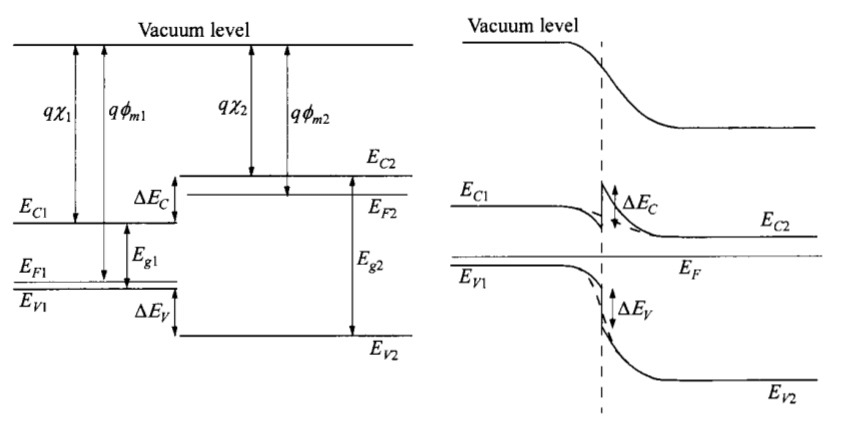
\includegraphics[width=6cm]{src/P-n-heterojunction-formation-Energy-bands-diagram-of-two-different-semiconductors.png}
    \caption{Energy bands of heterojunctions.}
    \label{fig:energy_bands_hetero}
\end{figure}
The energy band in a heterojunction undergoes a merging as in \cref{fig:energy_bands_hetero}. The injection ratio is higher in a heterojunction, which can be shown equal to
\[ \frac{j_e}{j_n} = \exp\brac{\frac{\pare{E_g}\+_N_ - \pare{E_g}\+_P_}{k\+_B_T}}. \]
\par
Heterojunctions may also be used in solar cells thanks to the window effect.

% subsubsection heterojunction (end)

\subsubsection{Non-Crystalline Semiconductors} % (fold)
\label{ssub:non_crystalline_semiconductors}

\paragraph{Doping} % (fold)
\label{par:doping}

In non-crystalline semiconductors, only a portion of the dopants act as donors or acceptors. Only if the electrons from the donors fill the impurities of the non-crystalline semiconductor will the Fermi energy be shifted and the density of electrons in the conduction band be raised.

% paragraph doping (end)

\paragraph{DC Conductivity} % (fold)
\label{par:dc_conductivity}

The transition of a electron from one localized state to another relies on the electron-lattice interaction. The rate of the transition is given by
\[ P = \nu\+_ph_e^{-2\alpha R}e^{-W/\pare{k\+_B_T}}, \]
where $\nu\+_ph_$ represents the frequency of the phonons, $e^{-2\alpha R}$ stands for the effect from the overlap of the wavefunctions, and $W$ is the average energy required to perform the hopping. The diffusion coefficient is given by
\[ D = PR^2, \]
where $R$ is the average displacement of each hopping.
\par
To DC conductivity is given by
\[ \inlinefinaleq{\sigma = \sigma_0 e^{-E/\pare{k\+_B_T}} + \sigma_1 e^{-E_1/\pare{k\+_B_T}} + \sigma_2 e^{-E_2/\pare{k\+_B_T}},} \]
where the three items on the RHS stands for the contribution from the extended states, the localized states from the tail of the band structure, and the localized state from the impurities.
\par
At low temperatures, variable-range hopping may dominates the conduction process, where we have
\[ \inlinefinaleq{\ln \sigma \propto T^{-1/4}.} \]

% paragraph dc_conductivity (end)

% subsubsection non_crystalline_semiconductors (end)

% subsection applications (end)

% section semiconductors (end)

\end{document}
